%!TEX root = ../../thesis.tex


\section{Post reduction stages}
\label{sec:posreduction}
From the {DRACS} pipeline the 1-D spectra of each target has been extracted.
However, the spectra still need to undergo some post-extraction steps.
In particular, wavelength calibration and telluric correction.
A detailed look of how these steps were developed and performed are addressed in the following section.

\subsection{Wavelength calibration}
\label{subsec:wavecalib}

Wavelength calibration is the process of assigning accurate wavelength values to each pixel in the spectra.
For {CRIRES} in the \nir{} this is challenging.
{CRIRES} uses a Thorium-Argon (\thar) lamp to place 6 emission spectra on the detector using fibres.
The spectra of the \thar{} emission lines are used to determine the spatial distribution of the wavelength solution across each detector using correlation with a spectral template.
\change{fix-up get a good citation, number of lines}{}\thar{} lamps are excellent at optical wavelengths where the numerous spectral lines enable precision of sub\,-\mps{} radial velocity measurements {HARPS} spectrograph.
For example the new ESPRESSO spectrograph uses \(\sim8600\) \thar{} lines\reference{paper for harps \thar{} lines}{(?)}.
However in the \nir{}, there is a relatively low density of \thar{} lines~\citep{kerber_laboratory_2009}, which, in combination with the alignment of the narrow wavelength range of the detector, causes a poor wavelength calibration to be obtained (e.g.\ {CRIRES}-POP~\citep{nicholls_crirespop_2017}).
Above 2.2\um{} there are {O-H} sky lines that can be used for wavelength calibration but for our observations below 2.2\um{} they are too dim.\reference{cite crires manual, and a paper about sky lines?}

These wavelength calibration issues were experienced when using the {ESO} {CRIRES} pipeline, with non-\thar{} features sometimes affecting the correlation.

Between the wavelength range 2.1--2.17\um{} there are roughly 80 \thar{} lines across all four detectors, as seen in \cref{fig:caliblamps}.
The {DRACS} pipeline does not use the \thar{} lamp files for wavelength calibration and leaves this as a post reduction step.

A common method for wavelength calibration that does not rely on \thar{} lamps of {CRIRES} involves using the telluric lines present to provide the wavelength solution~\citep[e.g.][]{brogi_signature_2012,brogi_carbon_2014,dekok_detection_2013}{\red{}~\citep{piskorz_evidence_2016}}.
This is made possible by the use of high resolution spectra, in which the telluric lines are well resolved, as well as accurate spectral information of the atmosphere.

We follow this method using the telluric absorption lines present in each observation as the wavelength reference.
Instead of directly using the {HITRAN} database~\citep{rothman_hitran2012_2013} for the telluric line positions~\citet[such as in][]{brogi_signature_2012,brogi_carbon_2014,dekok_detection_2013}, we use the {TAPAS} atmospheric transmission models~\citep{bertaux_tapas_2014} obtained for each observation.
The {TAPAS} models use the {HITRAN} database but also includes atmospheric profiles and physical meteorological measurements to model the telluric absorption strength.

To calibrate the wavelength the telluric lines in the model need to be associated to the corresponding telluric lines in the observed spectrum.
The centroid\footnote{Centre of the line} of each telluric line in the model is obtained by fitting the telluric transmission spectrum, \(T(\lambda)\), as a simple sum of Gaussian functions (subtracted from the continuum):
\begin{equation}
T(\lambda) = 1 - {\Sigma}_{i}\ G(\lambda, A_{i}, {\mu}_{i}, {\sigma}_{i}),
\end{equation}
where \(G\) is a Gaussian function of the form
\begin{equation}
G(\lambda, A, \mu, \sigma) = {A \textrm{e}}^{{-(\lambda-\mu)}^{2}/2\sigma^{2}},
\end{equation}
and \(A\), \(\mu\), \(\sigma\) are the amplitude, central wavelength, and standard deviation for each line respectively.
Telluric lines actually have a Voigt profile\footnote{A Voigt profile is a convolution of two broadening profiles, a Gaussian and a Lorentzian.
Gaussian broadening results from thermal Doppler broadening, and instrumental broadening while the Lorentzian broadening comes from molecular vibrational bands\citep{meier_art_2005}.} although they are not fully resolved in the \nir{} and their shape is dominated by the instrumental profile. \citet{seifahrt_synthesising_2010} measured the instrumental profile of {CRIRES} using singular-value decomposition and showed that it is extremely well represented by a single Gaussian below a \snr{} of around 300.
Therefore, wavelength calibration using single Gaussian fits to each line is sufficient.

The observed spectra contain two different spectral components: stellar and telluric lines, which are multiplied together: The observed spectra are therefore fitted with a multiplication of two Gaussian-sum models.
\begin{align}
I_{obs}(x) &= {I}_{tell}(x) \times {I}_{star}(x) \nonumber \\
I_{obs}(x) &= {\Big(1 - {\Sigma}_{j}\ G(x, A_{j}, {\mu}_{j}, {\sigma}_{j})\Big)}_{tell} \times {\Big(1 - {\Sigma}_{k} G(x, A_{k}, {\mu}_{k}, {\sigma}_{k})\Big)}_{star}, \label{eqn:obs}
\end{align}
where \(x\) is the pixel coordinates of the extracted spectra.

The identification between telluric and stellar lines is performed by hand for each spectra, using the telluric model as the reference.
Care was taken to fit the correct components to blended spectra where possible to improve the number telluric lines use for calibration.
The fits were inspected to ensure that they reasonably matched the line positions.
There was difficulty in identifying the shallow lines with depths below 1--2\%, but these were needed in some spectra to obtain a suitable fit.
If there were blended lines that did not appear to fit correctly they were not considered in the calibration step.

After fitting \(I_{obs}(x)\) to the observed spectrum and \(T(\lambda)\) to the telluric model the wavelength solution was obtained by fitting a second order polynomial to the centroid values \(\{\mu_{j}(x), \mu_{i}(\lambda)\}\) from the telluric components of the observed spectra and telluric model respectively.
A second order polynomial has been shown to be sufficient for higher precision {RV} studies~\citep[e.g.][]{bean_groundbased_2010, figueira_radial_2010}.
This polynomial is then used to map the whole spectrum from pixels into wavelength.
Higher \(3^{\textrm{rd}}\) and \(4^{\textrm{th}}\) order polynomials that are also used in the literature \citet[e.g.][]{seifahrt_synthesising_2010, ulmer-moll_telluric_2018} were attempted but had limited success here due to the limited number and uneven spacing of telluric lines in the narrow wavelength range analysed, especially on the second detector.
There were often large deviations due to the uneven spread of telluric lines, especially at the extremities.
Higher order terms for wavelength calibration are usually used in regions with a higher density of telluric lines and/or a longer wavelength span~\citep{piskorz_evidence_2016, seifahrt_synthesising_2010, ulmer-moll_telluric_2018}.

\begin{figure}
    \centering
    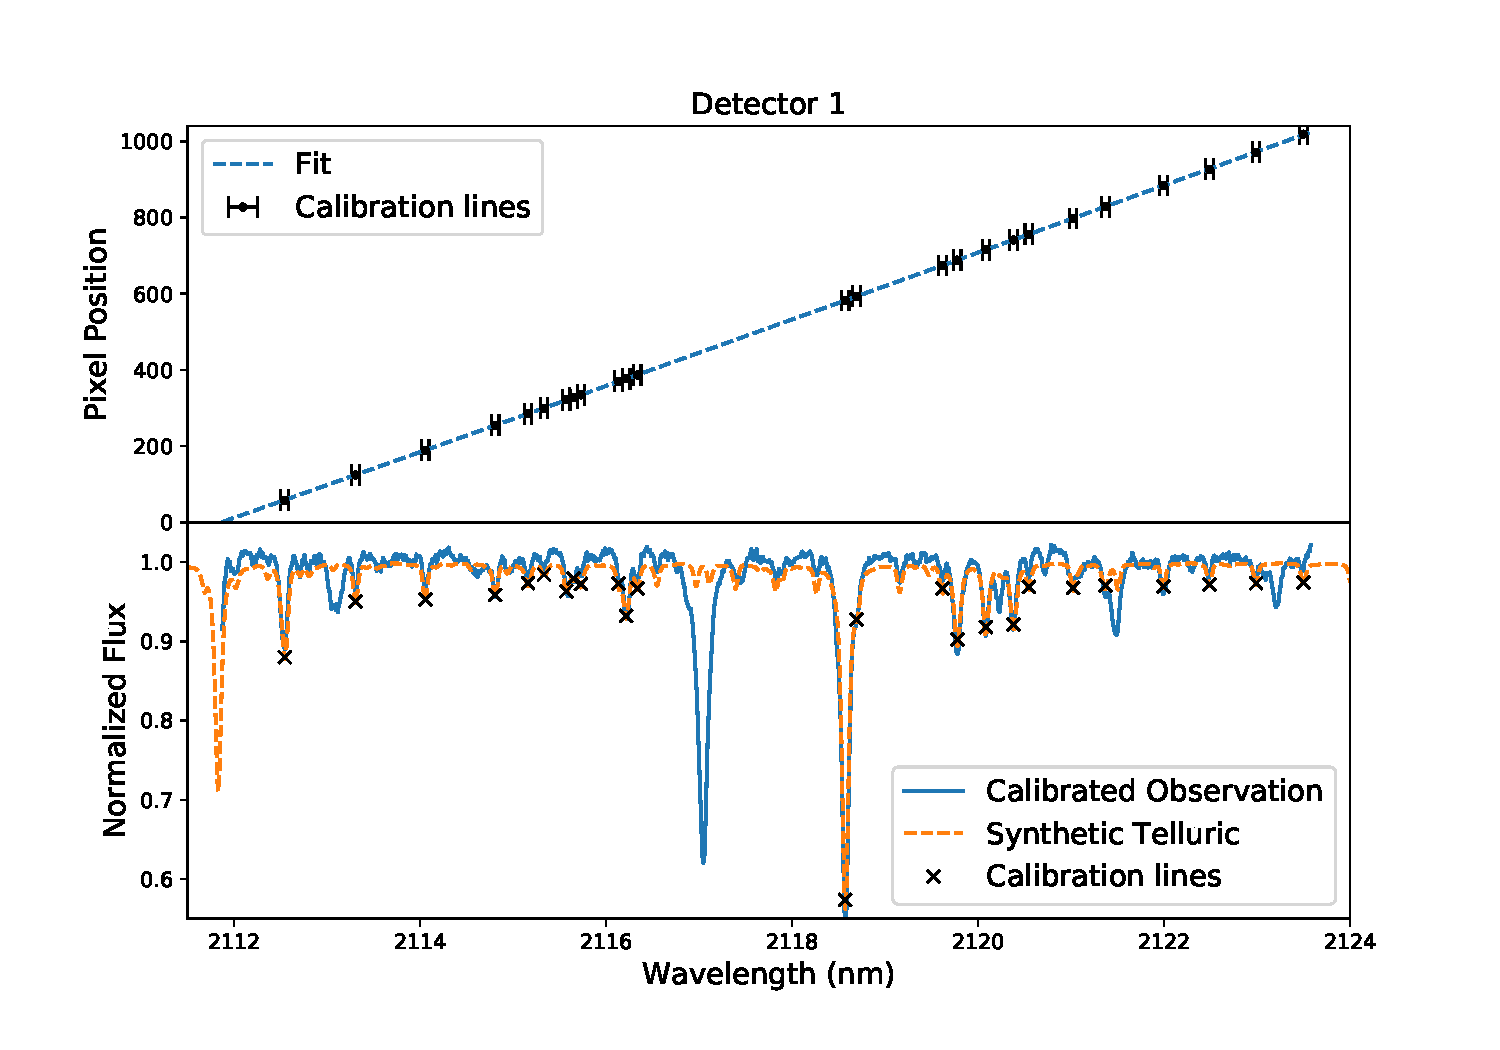
\includegraphics[width=0.8\linewidth]{figures/reduction/calibration.pdf}
    \caption{Wavelength calibration example.
    The equation of the fitted line for these points is $\lambda = -1.85e^{-7} x^2 + 1.16e^{-2} x + 2111.86$ with each coefficient shown to two decimal places only.
The horizontal error bars shown are the Gaussian line width, around 0.04\nm{}.}
    \label{fig:wl_calibration}
\end{figure}
\todo{explain the fit \cref{fig:wl_calibration}}

Much like with the \thar{} calibrations, this technique performs better when there is sufficient coverage of telluric lines on the detectors.
For the wavelength setting of these observations, the spectra from the second detector (top right panel of \cref{fig:spectraexamples}) only have two large telluric lines present with several small lines, with relative depths smaller than 1\%, which are often difficult to accurately identify.
This deteriorated the calibration stability for the second detector.
The second detector may have been ideal for the detection of a faint secondary spectra, with the lack of telluric contamination and stellar lines.
Unfortunately the wavelength calibration quality varies in an inverse way, being more difficult with few lines.

We note that there are many variations on this wavelength calibration technique including those integrated within programs such as \emph{TelFit}~\citet{gullikson_correcting_2014}, and {ESO}'s \emph{Molecfit}~\citet{smette_molecfit_2015}, that perform telluric correction and re-calibrate the wavelength axis themselves at the same time.

One improvement could have been to include a concurrent fitting of a stellar spectral model, adjusted for {RV}, along with the telluric model, could help to improve the wavelength calibration performed here. \citet{piskorz_evidence_2016} performed wavelength calibration using only a telluric line model at other \nir{} wavelengths {\red{} (e.g.\ 3.0--3.4\um{})}\todo{check value} successfully.
However, around 2\um{} they needed to include a fitted stellar model to obtain good wavelength calibration due to the weaker telluric lines in this region.
This is the same wavelength region of the data analysed here.
Having experience of performing wavelength calibration at other wavelengths may have revealed the difficulties of calibration from the telluric lines at 2\um{} sooner.

A brief attempt of wavelength calibration using the iterative calibration method outlined in~\cite{brogi_rotation_2016}.
This involved generating a set of quadratic wavelength solutions for the observed spectrum and cross-correlating each one against the telluric model.
The solutions for the next iteration are obtained by refining the parameters from the wavelength solution with the highest correlation.
The method worked well for~\citet{brogi_rotation_2016} as they included templates for both the star and telluric lines and they were observing in a wavelength domain in which there is a large number of strong and uniform stellar \ce{CO} lines across the detector.
Our brief experiments with this method were not successful as we did not include a stellar model or mask.
Without adding any stellar masking the telluric lines would strongly correlate to the stellar lines present, especially were there were blended lines.
This lead to visibly incorrect wavelength solutions and this method was abandoned.
If a stellar mask was used it may have been possible to achieve more sensible results, although still challenging to the low density of telluric lines at this wavelength range.


At one point it was considered to attempt a global fit of the wavelength calibration, using all four {CRIRES} detectors together.
This would create a consistent fit to the dispersion across all 4 detectors at once.
This would require extra fitting parameters to define the size of the 3 gaps between the detectors and any vertical offsets.
This fit may even need to be performed on the two-dimensional images, before the 1-D extraction.
This may have allowed for the telluric lines from neighbouring detectors to help fit the calibration on detectors were there are very few telluric lines (e.g.\ detector \#2).
The fitted instrument parameters such as the detector gaps may even be constrained so that they are physically consistent across all observations.
However, this idea was not explored further or implemented due to time constraints.

\missingfigure{Diagram of idea of combined detector fitting?}

An example of the wavelength calibration using all four detectors is provided in \cref{appendix:wavelength_fitting}.

In the future it may be possible or necessary to combine all of the methods above, including the \thar{} calibration lines, telluric models, stellar templates, and multiple detectors fitted at once to achieve precise wavelength calibration.

\begin{figure}
    \centering
    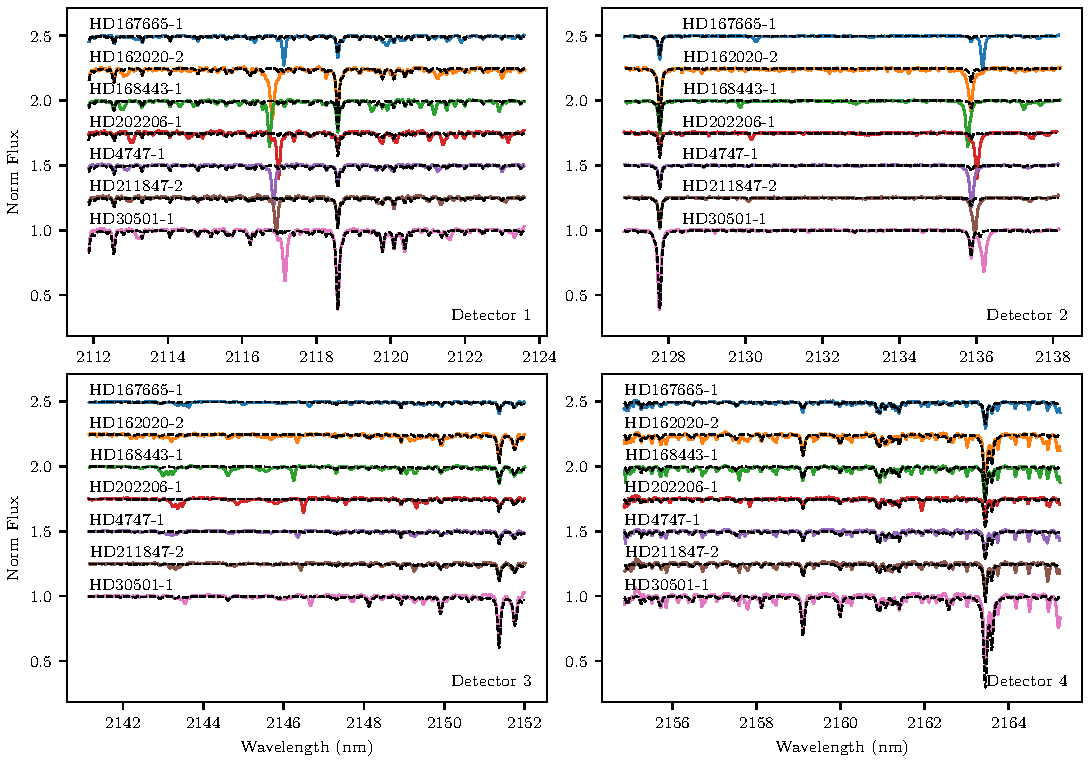
\includegraphics[width=1\linewidth]{figures/reduction/Spectra_examples}
    \caption{An example spectra for each target and each detector \#1--4 in order of increasing wavelength.
The solid lines are the spectra while the black dashed lines are the telluric models used for wavelength correction, showing good alignment with the spectra.}
    \label{fig:spectraexamples}
\end{figure}


\unfinished{See Solene's paper regarding Telluric correction with models and reference spectra}


In hindsight using the wavelength solution from the {ESO} pipeline may have been a good starting point, rather than the pixel positions, for calibration of the {DRACS} reduced spectra.
This may have made the line identification simpler.


\subsection{Telluric correction}



\subsection{Wavelength masking}
Throughout the course of this work several wavelength regions were found were we cannot reliably extract information, due to the wavelength calibration and telluric line corrections.
We apply different wavelength masks to these areas to remove them from the spectra.
The main reasons that wavelength masking is used are collated below.

Firstly, regions near the edges of each detector where the wavelength solution is extrapolated outside of the calibrating telluric lines are removed, reducing the effective size of each detector by about \(10\%\) or \(\sim100\) pixels.

Secondly, we mask out any remaining artefacts present in the spectra and the centres of deep telluric lines where telluric correction was not corrected properly, sometimes resulting in ``emission-like'' peaks in the corrected spectrum.
These factors combined result in masking out around a further 10\% of the observed spectra.

In \cref{sec:chi2_results} we also apply a further wavelength restriction to mask out regions where there is a large mismatch between the observed spectrum and the closest synthetic spectra to the host.
This significantly restricts the wavelength span utilized for that purpose to around only 43\%.
The masked regions created by this last mask are shown in \cref{fig:visualinspection-hd2118471}.


\unfinished{ADD non-\ce{H2O} fitting corrections.}

\missingfigure{Plots showing some examples the telluric correction with and without \ce{H2O} separated}

\subsection{Barycentric RV correction}
\label{{subsec:barycentriccorrection}}
After the telluric correction is performed, the spectra are corrected for Earth's barycentric motion. The orbital and rotational motion of the Earth imparts a daily and seasonal radial velocity measurement offset onto observations. To accurately compare the radial velocity (or spectral shift) between two measurements, they need to be translated into a common rest frame. The rest frame of choice is the barycentre of the Solar System.  Equations to relate the observed spectral shift to the RV shift at the \textit{Barycentric Celestial Reference Reference System}~\citep{rickman_transactions_2001} rest frame are provided in \citep{lindegren_fundamental_2003}.

In this work the barycentric velocity correction is calculated using PyAstronomy's\footnote{https://pyastronomy.readthedocs.io} \emph{helcor} function ported from the REDUCE IDL package (see~\citet[][]{piskunov_new_2002}).
This calculates radial velocity of the observer towards the astronomical target, accounting for Earth's barycentric motion as well as Earth's rotation.
This computation requires the date and time of the observation, the location of the observatory and the celestial coordinates of the target.
The observed spectra are Doppler shifted by the negative value of the barycentric velocity calculated, placing all spectra as if they were observed from the barycentre of the Solar System.

The maximum barycentric velocity of the Earth is around 30\kmps{}. It is common to see spectral regions $\pm30$\kmps{} either side of telluric lines with an absorption depth >2\% avoided in analysis (such as RV determination), as these will be affected by the telluric lines at some point in the year.
